\documentclass{article}
\usepackage{graphicx}
\usepackage{listings}
\lstset{breaklines=true}
\title{Technical Report for MIPS Processor Design}
\author{Webster Bei Yijie, yb44}
\begin{document}
	\maketitle
	\tableofcontents
	\newpage
	\section{Introduction}
	A five-stage MIPS ISA compatible microprocessor is implemented in Verilog using Intel Quartus. This report details the process that it took to implement the processor, and dive deep into the complications involved in dealing with various challenges encountered during the process. In the first section, I will briefly go through the different high-level components that the processor is made of. In the second section, I will go through the different groups of instructions that were implemented and how they were implemented. I will also talk about the way that testing was done and challenges that I encountered during the implementation of this microprocessor.  
	\section{Components}
		\subsection{ALU}
		ALU stands for arithmetic logic unit, and it is the most functional unit that we use to carry out many basic computations including addition, subtraction, logical and arithmetic shifts as well as logical and/or operations. Moreover, ALU is used to perform comparison between numbers where the comparison result could be used to determine whether a branch is taken when the processor encounters a conditional branch instruction. Other than addition and subtraction, most of these arithmetic operations are done simultaneously through individual component circuit within the ALU. Depending on the input which specifies what is needed from the computation, the ALU will then select the desired output from the group of outputs for each individual operation. \\
		The more cumbersome component of ALU is 32-bit signed integer adder. In my implementation, I used carry-lookahead implementation as opposed to the easier ripple carry adder for efficiency. The carry bits to the 31 1-bit full adder cells (all except the first bit which is cin) are generated using the carry lookahead generator cell module under the top level directory. 
		\begin{figure*}[h]
			\centering
			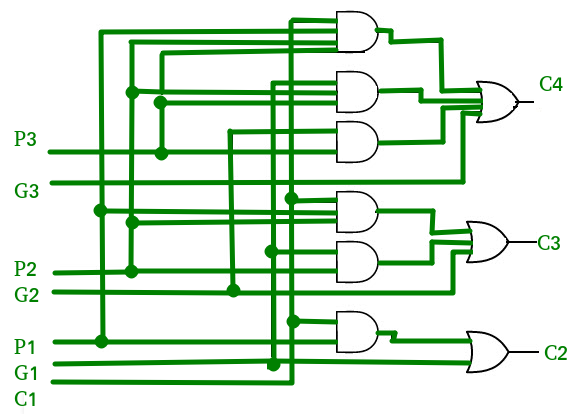
\includegraphics[width=3in]{cla}
		\end{figure*}
		\newpage
		The above figure shows part of the carry generation circuit. Since the circuit for generating carry for all 31 bits is way too complicated, I wrote a python script that outputs the structural Verilog code given number of bits needed. Similarly, the code used to generate the actual adder blocks is also produced indirectly by writing a Python script. For your reference, they are
		\subsection{Code for Generating Adder Verilog Code}
		\lstinputlisting[language=Python]{adderCodeGenerator.py}
		\subsection{Code for Generating Carry Lookahead Circuit Verilog Code}
		\lstinputlisting[language=Python]{carryGenerationCodeGenerator.py}
		Other significant parts of the ALU consist of Barrel Shifter implementation for the logical shift units.
		\begin{figure}[h]
			\centering
			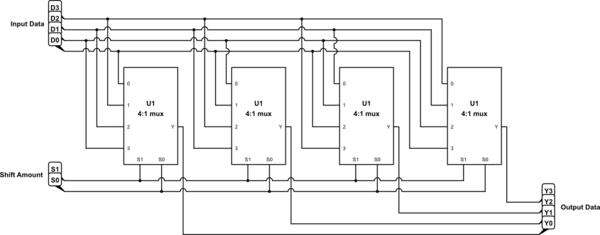
\includegraphics[width=5in]{barrel}
			\caption{Reference: https://electronics.stackexchange.com/questions/244129/barrel-shifter-using-multiplexer-how-to-go-about-it}
		\end{figure}
		The bitwise logical operations are implemented trivially using AND and OR gates for each input bit. In the very end, outputs from each of the arithmetic modules (i.e. logical operations, adders etc) are brought together to a MUX and the desired output is chosen based on the input ALU opcode.  
		\subsection{Register File}	
		The very fundamental building block of a register is d-flipflop which is implemented using behavior Verilog. Then 32 of those d-flipflop modules are strung together to generate a 32-bit register. Again, 32 of those register files are independently put together in a register file. A decoder that converts a 5 bit binary number into 32-bit one-hot signal implemented using pure combinational logic is used to produce write enable signal to the register that needs to be written, and used to produce \"pass-through" signals to tristate buffer controls to indicate which signals to let through. Tristate buffers are used instead of MUX for efficiency reasons since they significantly reduce the critical path length. 
		The Python script for generating the decoder Verilog code is:
		\subsection{Code for Generating Decoder Verilog Code}
		\lstinputlisting[language=Python]{DecoderGen.py}
		\subsection{Multiplication/Division Module}
		The multdiv circuit that performs multiplication and division is implemented in two separate modules, each performing the multiplication and division task independently. Both multiplication and division are done on signed 32-bit integers. Specifically, multiplication is done in 34 cycles (the first cycle is introduced for setting up the initial values error detection in edge cases) using Booth algorithm. The booth algorithm flow chart is
		\begin{figure}[!h]
			\centering
			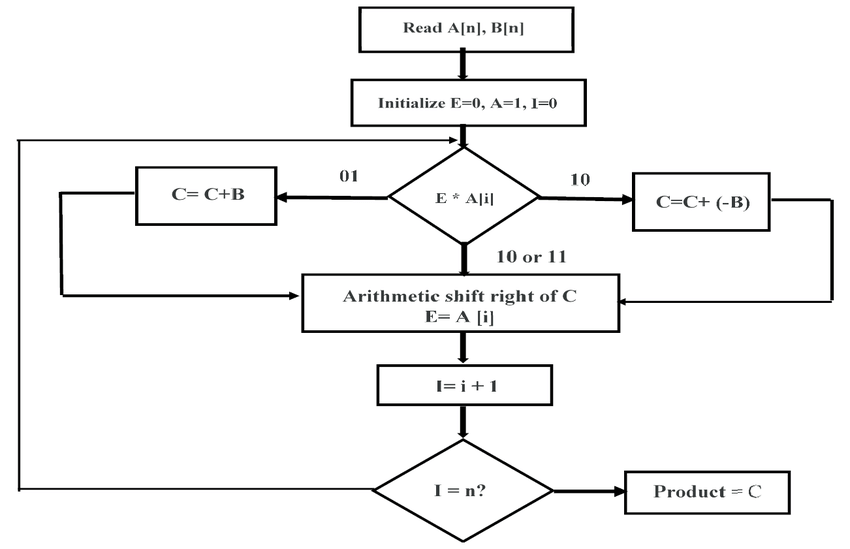
\includegraphics[width=4in]{booth}
			\caption{Reference: ResearchGate}
		\end{figure}
		Note that there is a counter involved in this process that determines where we are at in the multiplication process. Instead of using a generic adder for counting up, I used a 34-bit shift register which automatically moves the one hot bit from left to right with each clock tick. The location of the one-hot bit indicates our progress in the multiplication process. Similar counting procedure is done in the division module as well. \\
		The division is implemented using an unsigned integer division algorithm. Depending on the sign of the inputs, sign of the output number is then determined. A flow chart of the algorithm is included below.
		\begin{figure}[h]
			\centering
			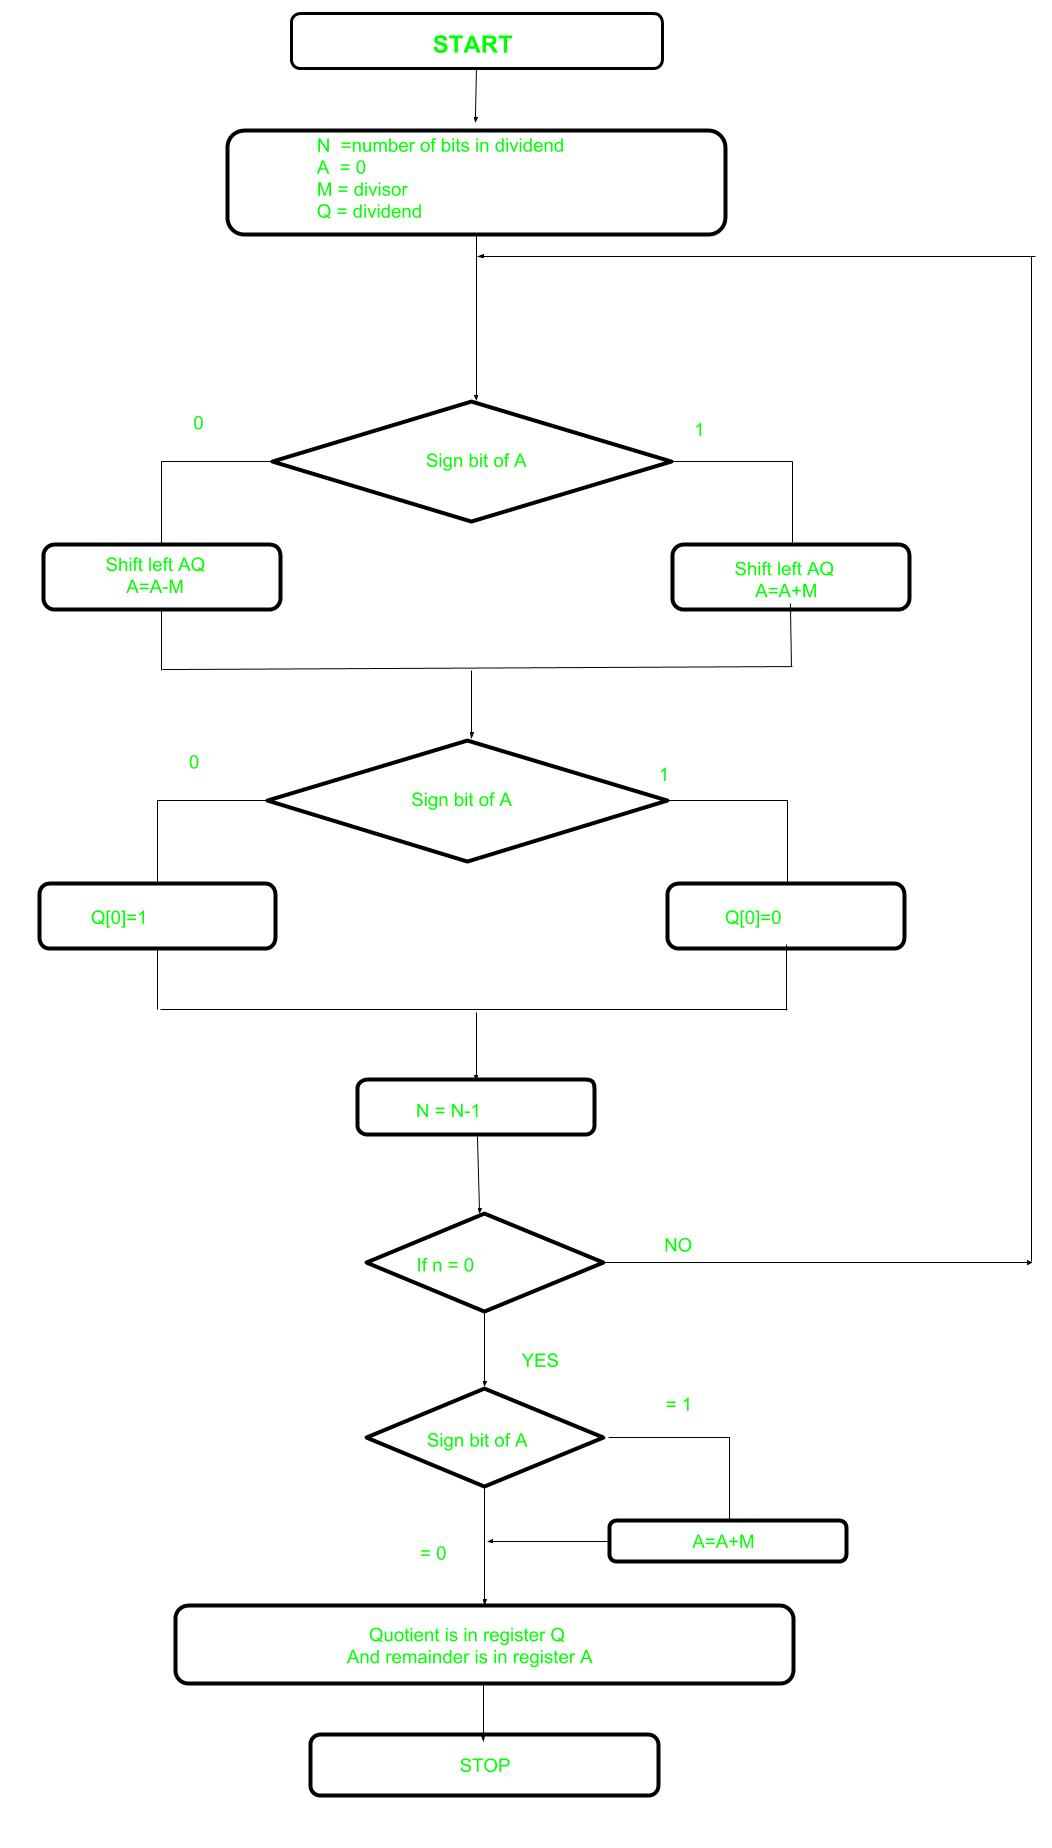
\includegraphics[width=4in, height=4in]{unsigned_division}
			\caption{Reference: GeeksForGeeks}
		\end{figure}
		The division process is done is 33 cycles as well, with the first cycle being the setup. The setup step includes taking the signs of input numbers and decide if a sign inversion is needed in the very end. I separated the setup step from the remaining steps because by doing so I can reduce the critical path length of the division process (taking out unnecessary MUX).
		\pagebreak
		\subsection{Memory Components}
		Memory components includes ROM(read only memory) that stores instructions and RAM(random access memory) that provides run-time data storage. Both modules are using the Quartus built-in modules created through the module creation wizard.
		\subsection{Control Logic}
		Control logic is the overarching module that coordinates the different individual modules. It has access to the data and instruction memory so that instructions can be read, decoded and executed. On a high level, this overarching module consists of 5 explicit stages each separated by a set of data latches. Different stages take control over different control signals that needs to be asserted at each stage as an instruction execute at that stage. I will dive into the details of how this is done in the next section. Overall, the structure of the processor pipeline looks exactly like the canonical 5 stage pipeline:
		\begin{figure}[h]
			\centering
			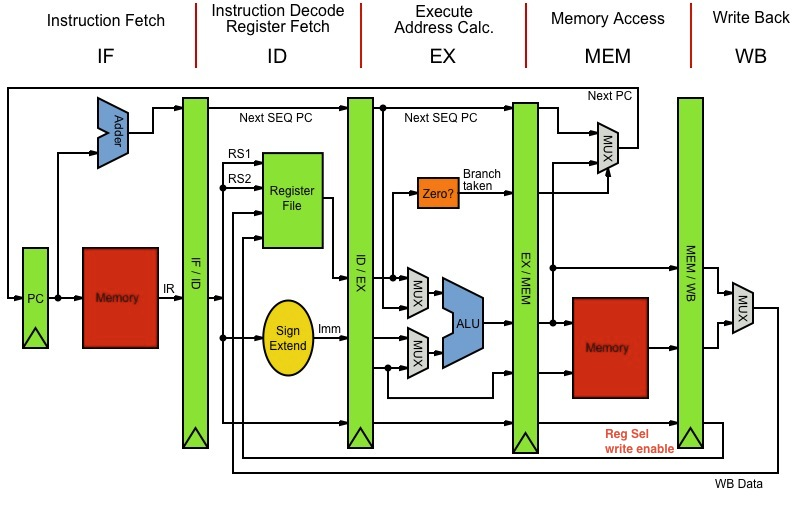
\includegraphics[width=5in]{pipeline}
			\caption{Reference: Stack Overflow}
		\end{figure}
	\section{Instruction Implementation}
		\subsection{Simple Arithmetics}
		The simple arithmetics are done using the ALU module implemented earlier. Since each ALU operation can be completed in a single cycle, the ALU module is simply put down as part of the execution stage and its output routed to the X/M latch. When the pipeline is first implemented, I ignored all the data dependencies and allowed all the single cycle operations to flow through the 5 stages of the pipeline. At the end of the pipeline, there is an extra adder unit for PC register value increment. Not too much needs to be taken care of at this stage. I will leave the majority of the complexity to be dealt with when we touch on bypassing. 
		\subsection{Multi-cycle Arithmetics}
		Unlike ALU operations, Multdiv operations cannot be completed in a single cycle. Therefore, I decided that it is easier to make the multiply and divide operations appear atomic to the pipeline. To achieve this, I used a d-flipflop to store the current status of the multdiv module to indicate whether it is busy currently when an instruction comes to the X stage. While the Multdiv module is busy calculating some results, I will hold the PC register and all the pipeline latches so that the instructions do not propagate through the pipeline when multiply or divide is in progress. 
		\subsection{Load Store}
		Noticing that each operation to the data memory takes takes two cycles to complete (i.e. when we pass in the address to be read in the first cycle, the data will be ready only in the next cycle), I decided that I should make the load and store instructions appear atomic to the pipeline as well (technically, only loads need to appear atomic, and stores in fact already behaves atomically). I used a d-flipflop to count to the next cycle before I allow the pipeline to move forward. The global stalling is similarly achieved by falsing the write enable at PC register and pipeline latches.
		\subsection{Branch}
		I implemented branching before implementing the bypass logic. Branching is achieved through the addition of a new full adder unit, which allows the target address to be calculated. Depending on the type of branch instructions, the target address is either taken directly from the instruction itself or computed from read register values. A gigantic MUX is used to choose the actual next PC where we read instructions from.
		\subsection{Bypassing}
		Bypassing logic and control signals are generated at X stage and M stage. At X stage, WX and MX bypassing are needed to replace the register values read from the register file with those that is ready to be written to the registers in the previous two instructions (i.e. instructions at M and W stages). My implementation first separates out the two types of instructions, one that reads RS values and one that reads RT or RD values. Some instructions belong to both. For operandA that goes into ALU and Multdiv, if any of the registers to be written at M and W is to be read by the current instruction at X, then I will directly take its value to replace my original operandA. It is slightly more complicated for operandB since operandB could come from RD or RS or even implicitly come from rstatus register, but the general structure is the same. The same is done for WM bypassing. One catch after full bypassing is that, we still need stall logic if we try to read a register immediately after the previous lw instruction produces it. This is done at the instruction fetch stage. In fetch stage, I predecode the instruction coming in to see if it is dependent on the previous lw instruction. If it does, then PC register is stalled for one cycle. I do not stall the F/D latch. Instead, a NOP instruction (32-bit 0s) is inserted into the F/D latch since it does nothing anyway. 
	\section{Testing}
	Testing is pretty difficult because anything inside the processor module needs to be wired to the top-entry module to be outputted. There also appears to be no easy way to directly observe the dmem and register file states. Therefore, it makes sense to perform unit test to dmem and register files, and trust that they work given the correct input to these modules. After making sure of that, I'm only observing the write enable signal and data signals to know that these two modules work correctly. Additionally, I added a 64bit output to the skeleton, and also as an output port for my processor. This 64bit output can be wired to any internal data within the processor so that I can observe its value at any cycle (effectively a print statement). This has been very helpful in the debugging process. \\
	Other than that, most of the testing and debugging is done by manually writing MIPS code, compile with assembulator and load to the simulator for waveform test. Control signals are routed to waveform output so that I can observe if registers and data are written correctly. I attempted to come up with general test cases (list of MIPS instructions) that covers different types of instructions, and ones that mixes those instructions. 
	\section{Challenges}
	I have encountered many different challenges when working on this processor. Upon reflection, I realize that most of the issue arise at the junction where adhoc sequential logic is needed. Although each different components can be thought of as a standalone finite state machine, it is unpractical to actually go through the process of creating finite state machines when implementing them. As such, it  is very important to develop some intuition for what to do in some of the common cases. \\
	One of the challenges that I encountered and later realized that there is a general solution frame to is where I needed to make something appear atomic to the outside world (e.g. the multdiv integration into processor). To achieve this goal, I used a register to store the state of the multiplication process, freeze the outside world until the state register tells me that I can unfreeze them. Other than that, the important thing is to generate signals that triggers the busy state and end the busy state. In the case of the multdiv, the mul or div instruction is the trigger and the result ready signal is the ending signal. Such a framework has been my approach to some other challenges I encountered as well. For example, in the implementation of multiplier and divisor units. \\
	Another challenge occurred when I was testing my register file implementation as I integrated it into the processor. My register file seems to produce incorrect values when the clock frequency is too high (period $<$ 5ns). Although the frequency at which it performs incorrectly is way beyond the specified 50MHz, it is still weird that the provided regfile module written in behavior Verilog does not have this issue. 
	\section{Conclusion}
	Overall, the 5 stage MIPS processor works and with full bypassing implemented, it is adequately efficient. There are areas where I believe I have used more than optimal amount of logic gates but those redundancy does not seem to hurt either the correctness nor the efficiency on the high level design. There is no known issues that I was able to find during my testings.
\end{document}
